\documentclass[11pt]{article}
\title{\textbf{Meccano fox-surd frame}}
\author{https://github.com/heptagons/meccano/frames/fox-surd}
\date{}

\usepackage{../../meccano}
\usepackage{tikz}
\usetikzlibrary{calc}

\begin{document}

\maketitle
\begin{abstract}
Meccano\meccanoref fox-surd frame is a generalization of fox-frame\footnote{
\href{https://github.com/heptagons/meccano/blob/main/frames/fox/fox.pdf}{Meccano fox frame }}
where two of the original five strips are no longer integers but surds which must be solved
using several more strips.
\end{abstract}

\section{Pentagons fox-surd}

\begin{figure}[h]
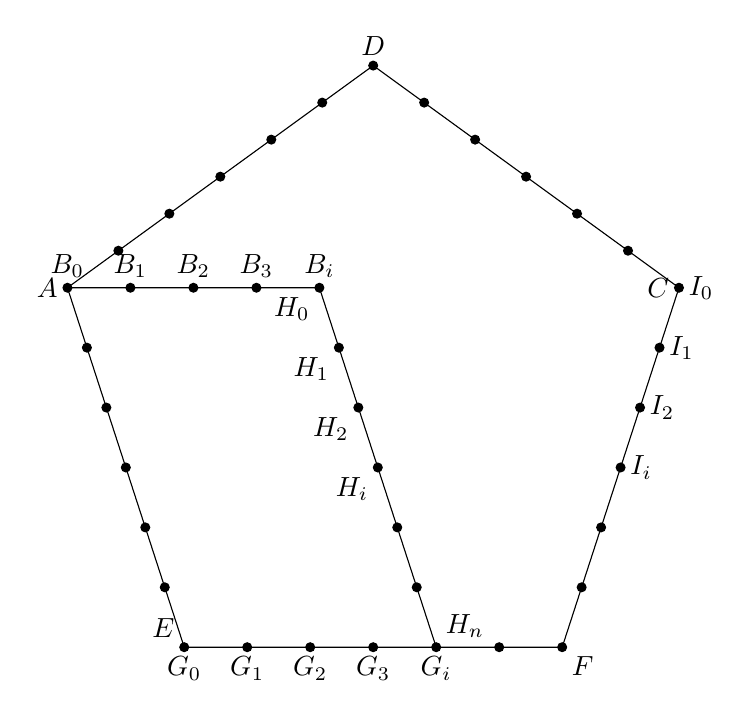
\begin{tikzpicture}
\begin{scope}[scale=0.8]
\begin{scope}
\draw[fill=black] (0,0) circle(2pt) node[above]{$B_0$}
-- ++(1,0) circle(2pt) node[above]{$B_1$}
-- ++(1,0) circle(2pt) node[above]{$B_2$}
-- ++(1,0) circle(2pt) node[above]{$B_3$}
-- ++(1,0) circle(2pt) node[above]{$B_i$} node[below left]{$H_0$}
-- ++(-72:1) circle(2pt) node[below left]{$H_1$}
-- ++(-72:1) circle(2pt) node[below left]{$H_2$}
-- ++(-72:1) circle(2pt) node[below left]{$H_i$}
-- ++(-72:1) circle(2pt)
-- ++(-72:1) circle(2pt)
-- ++(-72:1) circle(2pt) node[above right]{$H_n$} node[below]{$G_i$}
-- ++(-1,0) circle(2pt) node[below]{$G_3$}
-- ++(-1,0) circle(2pt) node[below]{$G_2$}
-- ++(-1,0) circle(2pt) node[below]{$G_1$}
-- ++(-1,0) circle(2pt) node[below]{$G_0$} node[above left]{$E$}
-- ++(108:1) circle(2pt)
-- ++(108:1) circle(2pt)
-- ++(108:1) circle(2pt)
-- ++(108:1) circle(2pt)
-- ++(108:1) circle(2pt)
-- ++(108:1);
\draw[fill=black] (0,0) node[left]{$A$}
-- ++(36:1) circle(2pt)
-- ++(36:1) circle(2pt)
-- ++(36:1) circle(2pt)
-- ++(36:1) circle(2pt)
-- ++(36:1) circle(2pt)
-- ++(36:1) circle(2pt) node[above]{$D$}
-- ++(-36:1) circle(2pt)
-- ++(-36:1) circle(2pt)
-- ++(-36:1) circle(2pt)
-- ++(-36:1) circle(2pt)
-- ++(-36:1) circle(2pt)
-- ++(-36:1) circle(2pt) node[left]{$C$} node[right]{$I_0$}
-- ++(-108:1) circle(2pt) node[right]{$I_1$}
-- ++(-108:1) circle(2pt) node[right]{$I_2$}
-- ++(-108:1) circle(2pt) node[right]{$I_i$}
-- ++(-108:1) circle(2pt)
-- ++(-108:1) circle(2pt)
-- ++(-108:1) circle(2pt) node[below right]{$F$}
-- ++(-1,0) circle(2pt)
-- ++(-1,0);

\end{scope}
\end{scope}
\end{tikzpicture}
\caption{Pentagon fox-surd.}
\label{fig:pentagon}
\end{figure}

\end{document}